% Options for packages loaded elsewhere
\PassOptionsToPackage{unicode}{hyperref}
\PassOptionsToPackage{hyphens}{url}
%
\documentclass[
]{article}
\usepackage{amsmath,amssymb}
\usepackage{iftex}
\ifPDFTeX
  \usepackage[T1]{fontenc}
  \usepackage[utf8]{inputenc}
  \usepackage{textcomp} % provide euro and other symbols
\else % if luatex or xetex
  \usepackage{unicode-math} % this also loads fontspec
  \defaultfontfeatures{Scale=MatchLowercase}
  \defaultfontfeatures[\rmfamily]{Ligatures=TeX,Scale=1}
\fi
\usepackage{lmodern}
\ifPDFTeX\else
  % xetex/luatex font selection
\fi
% Use upquote if available, for straight quotes in verbatim environments
\IfFileExists{upquote.sty}{\usepackage{upquote}}{}
\IfFileExists{microtype.sty}{% use microtype if available
  \usepackage[]{microtype}
  \UseMicrotypeSet[protrusion]{basicmath} % disable protrusion for tt fonts
}{}
\makeatletter
\@ifundefined{KOMAClassName}{% if non-KOMA class
  \IfFileExists{parskip.sty}{%
    \usepackage{parskip}
  }{% else
    \setlength{\parindent}{0pt}
    \setlength{\parskip}{6pt plus 2pt minus 1pt}}
}{% if KOMA class
  \KOMAoptions{parskip=half}}
\makeatother
\usepackage{xcolor}
\usepackage[margin=1in]{geometry}
\usepackage{longtable,booktabs,array}
\usepackage{calc} % for calculating minipage widths
% Correct order of tables after \paragraph or \subparagraph
\usepackage{etoolbox}
\makeatletter
\patchcmd\longtable{\par}{\if@noskipsec\mbox{}\fi\par}{}{}
\makeatother
% Allow footnotes in longtable head/foot
\IfFileExists{footnotehyper.sty}{\usepackage{footnotehyper}}{\usepackage{footnote}}
\makesavenoteenv{longtable}
\usepackage{graphicx}
\makeatletter
\def\maxwidth{\ifdim\Gin@nat@width>\linewidth\linewidth\else\Gin@nat@width\fi}
\def\maxheight{\ifdim\Gin@nat@height>\textheight\textheight\else\Gin@nat@height\fi}
\makeatother
% Scale images if necessary, so that they will not overflow the page
% margins by default, and it is still possible to overwrite the defaults
% using explicit options in \includegraphics[width, height, ...]{}
\setkeys{Gin}{width=\maxwidth,height=\maxheight,keepaspectratio}
% Set default figure placement to htbp
\makeatletter
\def\fps@figure{htbp}
\makeatother
\setlength{\emergencystretch}{3em} % prevent overfull lines
\providecommand{\tightlist}{%
  \setlength{\itemsep}{0pt}\setlength{\parskip}{0pt}}
\setcounter{secnumdepth}{-\maxdimen} % remove section numbering
\usepackage{fontspec}
\setmainfont{NanumGothic}
\ifLuaTeX
  \usepackage{selnolig}  % disable illegal ligatures
\fi
\usepackage{bookmark}
\IfFileExists{xurl.sty}{\usepackage{xurl}}{} % add URL line breaks if available
\urlstyle{same}
\hypersetup{
  pdftitle={Quiz 250407 (Which World?)},
  pdfauthor={coop711},
  hidelinks,
  pdfcreator={LaTeX via pandoc}}

\title{Quiz 250407 (Which World?)}
\author{coop711}
\date{2025-04-19 10:30:53}

\begin{document}
\maketitle

\section{6주차 데이터 실험
집계}\label{uxc8fcuxcc28-uxb370uxc774uxd130-uxc2e4uxd5d8-uxc9d1uxacc4}

\subsection{실험의 목적}\label{uxc2e4uxd5d8uxc758-uxbaa9uxc801}

6주차 구글 예습 설문지 집계결과를 분석합니다.

Q1\textasciitilde Q6에서는 랜덤화의 효과로 Red, Black 이 얼마나 닮았는지
알아봅니다.

Q7에서는 소득의 절대값보다 상대적 비교가 중시된다는 실험 결과를
분석합니다.

제출시간의 분포가 날마다 고른지, Red, Black 간에는 닮았는지 알아봅니다.

\subsubsection{Red, Black을 잘못 표시한
사람들}\label{red-blackuxc744-uxc798uxbabb-uxd45cuxc2dcuxd55c-uxc0acuxb78cuxb4e4}

\begin{longtable}[]{@{}
  >{\centering\arraybackslash}p{(\columnwidth - 6\tabcolsep) * \real{0.3056}}
  >{\centering\arraybackslash}p{(\columnwidth - 6\tabcolsep) * \real{0.1528}}
  >{\centering\arraybackslash}p{(\columnwidth - 6\tabcolsep) * \real{0.2083}}
  >{\centering\arraybackslash}p{(\columnwidth - 6\tabcolsep) * \real{0.2083}}@{}}
\toprule\noalign{}
\begin{minipage}[b]{\linewidth}\centering
제출시간
\end{minipage} & \begin{minipage}[b]{\linewidth}\centering
학번
\end{minipage} & \begin{minipage}[b]{\linewidth}\centering
랜덤화출석부
\end{minipage} & \begin{minipage}[b]{\linewidth}\centering
구글예습퀴즈
\end{minipage} \\
\midrule\noalign{}
\endhead
\bottomrule\noalign{}
\endlastfoot
2025-04-13 21:41:05 & 20202133 & Red & Black \\
2025-04-13 21:50:35 & 20241011 & Red & Black \\
\end{longtable}

\begin{longtable}[]{@{}
  >{\raggedright\arraybackslash}p{(\columnwidth - 4\tabcolsep) * \real{0.3611}}
  >{\centering\arraybackslash}p{(\columnwidth - 4\tabcolsep) * \real{0.2778}}
  >{\centering\arraybackslash}p{(\columnwidth - 4\tabcolsep) * \real{0.3056}}@{}}
\toprule\noalign{}
\begin{minipage}[b]{\linewidth}\raggedright
~
\end{minipage} & \begin{minipage}[b]{\linewidth}\centering
Red(구글예습퀴즈)
\end{minipage} & \begin{minipage}[b]{\linewidth}\centering
Black(구글예습퀴즈)
\end{minipage} \\
\midrule\noalign{}
\endhead
\bottomrule\noalign{}
\endlastfoot
\textbf{Red(랜덤화출석부)} & 187 & 2 \\
\textbf{Black(랜덤화출석부)} & 0 & 183 \\
\textbf{계} & 187 & 185 \\
\end{longtable}

랜덤화출석부에 있는 Red, Black 과 실제 구글설문에 올린 Red, Black 이
다른 사람들의 수효는 2명입니다.

Red를 Black 이라고 한 사람이 2명, Black 을 Red 라고 한 사람이 0명입니다.

두 가지 방법으로 분석합니다.

우선 Red, Black 을 잘못 선택한 2명을 랜덤하게 둘로 나누면 어느 한 쪽
집단에 들어갈 기대인원은 2명을 둘로 나눈 1(명)이고, 표준오차는 2의
제곱근에 1/2을 곱해 준 0.7명이 됩니다.

실제로 Red를 Black 이라고 한 사람수, 2명이나 Black 을 Red 라고 한
사람수, 0명은 기대인원으로부터 표준오차 범위는 벗어 나지만 표준오차 두
배 범위에는 잘 들어갑니다.

두 번째 분석 방법은 확률을 계산해 보는 것입니다.

Red, Black 을 잘못 선택한 2명을 랜덤하게 둘로 나눌 때, 실제로 관찰된 2명
이상이나 0명이하로 잘못 선택한 사람수가 나올 가능성은 얼마나 되는가
입니다.

이 경우 공평한 동전던지기를 확률 법칙으로 표현한 이항분포로부터 계산할
수 있습니다.

시행횟수가 2이고 한 번 시행에서 성공확률이 1/2 인 이항분포에서
성공횟수가 0이하이거나 2이상을 관찰할 확률은 0.5입니다.

공평한 동전 던지기에서 앞면이 0개 이하 나오는 확률은 2개 이상 나오는
확률과 같기 때문에 사실상 한쪽만 계산해서 2배 해 주면 됩니다.

이 값을 p-value 라고 하는데, p-value가 0.05보다 작을 때
\textbf{통계적으로 유의한 차이를 관찰}하였다고 말합니다.

즉, 공평한 동전을 던지는 것과 같은 과정이라고 가정하였을 때 실제로
관찰된 값들이 가정으로부터 얼마나 떨어져 있는지를 표현한 것입니다.

0.05는 이런 실험을 스무 번 정도 반복하면 1번 나올 정도로 드문 사건을
의미합니다.

즉 가정이 잘못되었다는 것입니다.

그런데 Red, Black 을 잘못 표시한 사람들의 분포에서 관찰된 p-value 는
0.05와는 비교도 안될 정도로 큰 값입니다.

따라서 두 집단이 랜덤화 효과가 작동하여 \textbf{통계적으로 유의한 차이를
보이지 않는다}고 할 수 있습니다.

\subsubsection{응답인원의 Red,
Black}\label{uxc751uxb2f5uxc778uxc6d0uxc758-red-black}

Red 로 응답한 인원은 187명, Black 에 응답한 인원은 185명입니다.

전체 응답인원 372 명을 랜덤하게 둘로 나눌 때 어느 한 쪽의 기대인원은
전체 응답인원의 절반인 186명이고, 표준오차는 전체 응답인원의 제곱근에
1/2을 곱해 준 9.6 명입니다.

따라서 Red, Black 각 그룹에 관찰된 인원은 기대인원으로부터 표준오차 범위
안에 들어갑니다.

\subsection{Q1. 월간 독서율}\label{q1.-uxc6d4uxac04-uxb3c5uxc11cuxc728}

\begin{flushleft}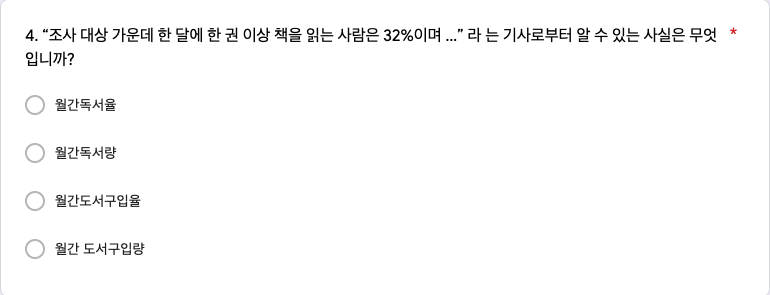
\includegraphics[width=0.75\linewidth]{./pics/Quiz210330_Q4} \end{flushleft}

\subsubsection{집계}\label{uxc9d1uxacc4}

\begin{longtable}[]{@{}
  >{\raggedright\arraybackslash}p{(\columnwidth - 10\tabcolsep) * \real{0.1519}}
  >{\centering\arraybackslash}p{(\columnwidth - 10\tabcolsep) * \real{0.1646}}
  >{\centering\arraybackslash}p{(\columnwidth - 10\tabcolsep) * \real{0.1646}}
  >{\centering\arraybackslash}p{(\columnwidth - 10\tabcolsep) * \real{0.2152}}
  >{\centering\arraybackslash}p{(\columnwidth - 10\tabcolsep) * \real{0.2278}}
  >{\centering\arraybackslash}p{(\columnwidth - 10\tabcolsep) * \real{0.0759}}@{}}
\toprule\noalign{}
\begin{minipage}[b]{\linewidth}\raggedright
~
\end{minipage} & \begin{minipage}[b]{\linewidth}\centering
월간독서율
\end{minipage} & \begin{minipage}[b]{\linewidth}\centering
월간독서량
\end{minipage} & \begin{minipage}[b]{\linewidth}\centering
월간도서구입율
\end{minipage} & \begin{minipage}[b]{\linewidth}\centering
월간 도서구입량
\end{minipage} & \begin{minipage}[b]{\linewidth}\centering
계
\end{minipage} \\
\midrule\noalign{}
\endhead
\bottomrule\noalign{}
\endlastfoot
\textbf{Red} & 162 & 18 & 6 & 1 & 187 \\
\textbf{Black} & 161 & 21 & 3 & 0 & 185 \\
\textbf{계} & 323 & 39 & 9 & 1 & 372 \\
\end{longtable}

\begin{longtable}[]{@{}
  >{\raggedleft\arraybackslash}p{(\columnwidth - 4\tabcolsep) * \real{0.2361}}
  >{\raggedleft\arraybackslash}p{(\columnwidth - 4\tabcolsep) * \real{0.0694}}
  >{\raggedleft\arraybackslash}p{(\columnwidth - 4\tabcolsep) * \real{0.1389}}@{}}
\caption{Pearson's Chi-squared test: \texttt{.}}\tabularnewline
\toprule\noalign{}
\begin{minipage}[b]{\linewidth}\raggedleft
Test statistic
\end{minipage} & \begin{minipage}[b]{\linewidth}\raggedleft
df
\end{minipage} & \begin{minipage}[b]{\linewidth}\raggedleft
P value
\end{minipage} \\
\midrule\noalign{}
\endfirsthead
\toprule\noalign{}
\begin{minipage}[b]{\linewidth}\raggedleft
Test statistic
\end{minipage} & \begin{minipage}[b]{\linewidth}\raggedleft
df
\end{minipage} & \begin{minipage}[b]{\linewidth}\raggedleft
P value
\end{minipage} \\
\midrule\noalign{}
\endhead
\bottomrule\noalign{}
\endlastfoot
2.223 & 3 & 0.5274 \\
\end{longtable}

Q1의 집계 결과가 Red, Black 간에 통계적으로 유의한 차이가 있는지
알아보기 위하여 카이제곱 테스트를 수행하였습니다.

그 결과 카이제곱 통계량은 2.22, 자유도는 3 , p-value 는 0.5274이므로
Red, Black 간에 통계적으로 유의한 차이를 보이고 있습니다.

어디가 문제인가요?

\subsubsection{\%}\label{section}

\begin{longtable}[]{@{}
  >{\centering\arraybackslash}p{(\columnwidth - 8\tabcolsep) * \real{0.1806}}
  >{\centering\arraybackslash}p{(\columnwidth - 8\tabcolsep) * \real{0.1806}}
  >{\centering\arraybackslash}p{(\columnwidth - 8\tabcolsep) * \real{0.2361}}
  >{\centering\arraybackslash}p{(\columnwidth - 8\tabcolsep) * \real{0.2500}}
  >{\centering\arraybackslash}p{(\columnwidth - 8\tabcolsep) * \real{0.1250}}@{}}
\toprule\noalign{}
\begin{minipage}[b]{\linewidth}\centering
월간독서율
\end{minipage} & \begin{minipage}[b]{\linewidth}\centering
월간독서량
\end{minipage} & \begin{minipage}[b]{\linewidth}\centering
월간도서구입율
\end{minipage} & \begin{minipage}[b]{\linewidth}\centering
월간 도서구입량
\end{minipage} & \begin{minipage}[b]{\linewidth}\centering
계
\end{minipage} \\
\midrule\noalign{}
\endhead
\bottomrule\noalign{}
\endlastfoot
86.83 & 10.48 & 2.42 & 0.27 & 100.00 \\
\end{longtable}

정답률은 Red, Black 을 합하여 계산하는데, 86.8(\%) 입니다.

\subsection{Q2. 지역 및 지역크기별 가구수 비례
무작위추출법}\label{q2.-uxc9c0uxc5ed-uxbc0f-uxc9c0uxc5eduxd06cuxae30uxbcc4-uxac00uxad6cuxc218-uxbe44uxb840-uxbb34uxc791uxc704uxcd94uxcd9cuxbc95}

\begin{flushleft}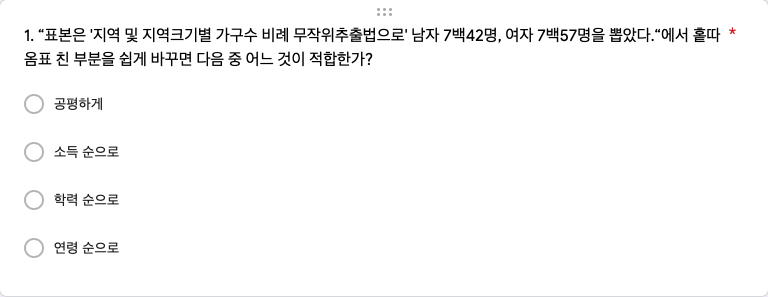
\includegraphics[width=0.75\linewidth]{./pics/Quiz210330_Q1} \end{flushleft}

\subsubsection{집계}\label{uxc9d1uxacc4-1}

\begin{longtable}[]{@{}
  >{\raggedright\arraybackslash}p{(\columnwidth - 10\tabcolsep) * \real{0.1667}}
  >{\centering\arraybackslash}p{(\columnwidth - 10\tabcolsep) * \real{0.1528}}
  >{\centering\arraybackslash}p{(\columnwidth - 10\tabcolsep) * \real{0.1944}}
  >{\centering\arraybackslash}p{(\columnwidth - 10\tabcolsep) * \real{0.1944}}
  >{\centering\arraybackslash}p{(\columnwidth - 10\tabcolsep) * \real{0.1944}}
  >{\centering\arraybackslash}p{(\columnwidth - 10\tabcolsep) * \real{0.0833}}@{}}
\toprule\noalign{}
\begin{minipage}[b]{\linewidth}\raggedright
~
\end{minipage} & \begin{minipage}[b]{\linewidth}\centering
공평하게
\end{minipage} & \begin{minipage}[b]{\linewidth}\centering
소득 순으로
\end{minipage} & \begin{minipage}[b]{\linewidth}\centering
학력 순으로
\end{minipage} & \begin{minipage}[b]{\linewidth}\centering
연령 순으로
\end{minipage} & \begin{minipage}[b]{\linewidth}\centering
계
\end{minipage} \\
\midrule\noalign{}
\endhead
\bottomrule\noalign{}
\endlastfoot
\textbf{Red} & 162 & 10 & 9 & 6 & 187 \\
\textbf{Black} & 171 & 6 & 3 & 5 & 185 \\
\textbf{계} & 333 & 16 & 12 & 11 & 372 \\
\end{longtable}

\begin{longtable}[]{@{}
  >{\raggedleft\arraybackslash}p{(\columnwidth - 4\tabcolsep) * \real{0.2361}}
  >{\raggedleft\arraybackslash}p{(\columnwidth - 4\tabcolsep) * \real{0.0694}}
  >{\raggedleft\arraybackslash}p{(\columnwidth - 4\tabcolsep) * \real{0.1389}}@{}}
\caption{Pearson's Chi-squared test: \texttt{.}}\tabularnewline
\toprule\noalign{}
\begin{minipage}[b]{\linewidth}\raggedleft
Test statistic
\end{minipage} & \begin{minipage}[b]{\linewidth}\raggedleft
df
\end{minipage} & \begin{minipage}[b]{\linewidth}\raggedleft
P value
\end{minipage} \\
\midrule\noalign{}
\endfirsthead
\toprule\noalign{}
\begin{minipage}[b]{\linewidth}\raggedleft
Test statistic
\end{minipage} & \begin{minipage}[b]{\linewidth}\raggedleft
df
\end{minipage} & \begin{minipage}[b]{\linewidth}\raggedleft
P value
\end{minipage} \\
\midrule\noalign{}
\endhead
\bottomrule\noalign{}
\endlastfoot
4.324 & 3 & 0.2286 \\
\end{longtable}

Q2의 집계 결과가 Red, Black 간에 통계적으로 유의한 차이가 있는지
알아보기 위하여 카이제곱 테스트를 수행하였습니다.

그 결과 카이제곱 통계량은 4.32, 자유도는 3, p-value 는 0.2286이므로 Red,
Black 간에 통계적으로 유의한 차이를 보이지 않습니다.

실제로 닮은 게 느껴집니까?

\subsubsection{\%}\label{section-1}

\begin{longtable}[]{@{}
  >{\centering\arraybackslash}p{(\columnwidth - 8\tabcolsep) * \real{0.1528}}
  >{\centering\arraybackslash}p{(\columnwidth - 8\tabcolsep) * \real{0.1944}}
  >{\centering\arraybackslash}p{(\columnwidth - 8\tabcolsep) * \real{0.1944}}
  >{\centering\arraybackslash}p{(\columnwidth - 8\tabcolsep) * \real{0.1944}}
  >{\centering\arraybackslash}p{(\columnwidth - 8\tabcolsep) * \real{0.1111}}@{}}
\toprule\noalign{}
\begin{minipage}[b]{\linewidth}\centering
공평하게
\end{minipage} & \begin{minipage}[b]{\linewidth}\centering
소득 순으로
\end{minipage} & \begin{minipage}[b]{\linewidth}\centering
학력 순으로
\end{minipage} & \begin{minipage}[b]{\linewidth}\centering
연령 순으로
\end{minipage} & \begin{minipage}[b]{\linewidth}\centering
계
\end{minipage} \\
\midrule\noalign{}
\endhead
\bottomrule\noalign{}
\endlastfoot
89.5 & 4.3 & 3.2 & 3.0 & 100.0 \\
\end{longtable}

정답률은 Red, Black 을 합하여 계산하는데, 89.5(\%) 입니다.

\subsection{Q3. 한달 독서량의
분포}\label{q3.-uxd55cuxb2ec-uxb3c5uxc11cuxb7c9uxc758-uxbd84uxd3ec}

\begin{flushleft}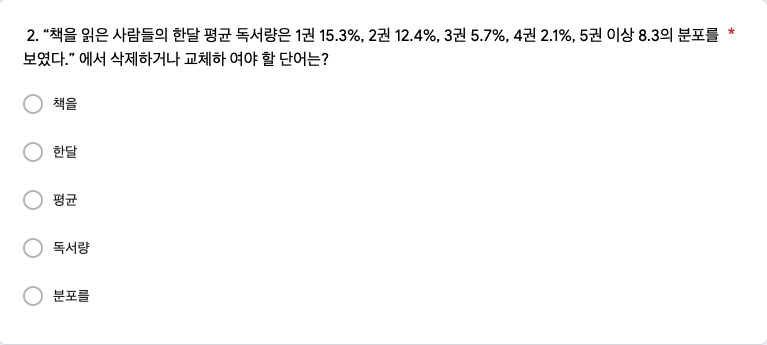
\includegraphics[width=0.75\linewidth]{./pics/Quiz210330_Q2} \end{flushleft}

\subsubsection{집계}\label{uxc9d1uxacc4-2}

\begin{longtable}[]{@{}
  >{\raggedright\arraybackslash}p{(\columnwidth - 12\tabcolsep) * \real{0.1667}}
  >{\centering\arraybackslash}p{(\columnwidth - 12\tabcolsep) * \real{0.0972}}
  >{\centering\arraybackslash}p{(\columnwidth - 12\tabcolsep) * \real{0.0972}}
  >{\centering\arraybackslash}p{(\columnwidth - 12\tabcolsep) * \real{0.0972}}
  >{\centering\arraybackslash}p{(\columnwidth - 12\tabcolsep) * \real{0.1250}}
  >{\centering\arraybackslash}p{(\columnwidth - 12\tabcolsep) * \real{0.1250}}
  >{\centering\arraybackslash}p{(\columnwidth - 12\tabcolsep) * \real{0.0833}}@{}}
\toprule\noalign{}
\begin{minipage}[b]{\linewidth}\raggedright
~
\end{minipage} & \begin{minipage}[b]{\linewidth}\centering
책을
\end{minipage} & \begin{minipage}[b]{\linewidth}\centering
한달
\end{minipage} & \begin{minipage}[b]{\linewidth}\centering
평균
\end{minipage} & \begin{minipage}[b]{\linewidth}\centering
독서량
\end{minipage} & \begin{minipage}[b]{\linewidth}\centering
분포를
\end{minipage} & \begin{minipage}[b]{\linewidth}\centering
계
\end{minipage} \\
\midrule\noalign{}
\endhead
\bottomrule\noalign{}
\endlastfoot
\textbf{Red} & 15 & 9 & 129 & 15 & 19 & 187 \\
\textbf{Black} & 8 & 4 & 113 & 23 & 37 & 185 \\
\textbf{계} & 23 & 13 & 242 & 38 & 56 & 372 \\
\end{longtable}

\begin{longtable}[]{@{}
  >{\raggedleft\arraybackslash}p{(\columnwidth - 4\tabcolsep) * \real{0.2361}}
  >{\raggedleft\arraybackslash}p{(\columnwidth - 4\tabcolsep) * \real{0.0694}}
  >{\raggedleft\arraybackslash}p{(\columnwidth - 4\tabcolsep) * \real{0.1667}}@{}}
\caption{Pearson's Chi-squared test: \texttt{.}}\tabularnewline
\toprule\noalign{}
\begin{minipage}[b]{\linewidth}\raggedleft
Test statistic
\end{minipage} & \begin{minipage}[b]{\linewidth}\raggedleft
df
\end{minipage} & \begin{minipage}[b]{\linewidth}\raggedleft
P value
\end{minipage} \\
\midrule\noalign{}
\endfirsthead
\toprule\noalign{}
\begin{minipage}[b]{\linewidth}\raggedleft
Test statistic
\end{minipage} & \begin{minipage}[b]{\linewidth}\raggedleft
df
\end{minipage} & \begin{minipage}[b]{\linewidth}\raggedleft
P value
\end{minipage} \\
\midrule\noalign{}
\endhead
\bottomrule\noalign{}
\endlastfoot
12.57 & 4 & 0.01357 * \\
\end{longtable}

Q3의 집계 결과가 Red, Black 간에 통계적으로 유의한 차이가 있는지
알아보기 위하여 카이제곱 테스트를 수행하였습니다.

그 결과 카이제곱 통계량은 12.57, 자유도는 4, p-value 는 0.0136이므로
Red, Black 간에 통계적으로 유의한 차이를 보이고(지) 있(않)습니다.

실제로 닮은 게 느껴집니까?

\subsubsection{\%}\label{section-2}

\begin{longtable}[]{@{}
  >{\centering\arraybackslash}p{(\columnwidth - 10\tabcolsep) * \real{0.0972}}
  >{\centering\arraybackslash}p{(\columnwidth - 10\tabcolsep) * \real{0.0972}}
  >{\centering\arraybackslash}p{(\columnwidth - 10\tabcolsep) * \real{0.0972}}
  >{\centering\arraybackslash}p{(\columnwidth - 10\tabcolsep) * \real{0.1250}}
  >{\centering\arraybackslash}p{(\columnwidth - 10\tabcolsep) * \real{0.1250}}
  >{\centering\arraybackslash}p{(\columnwidth - 10\tabcolsep) * \real{0.1250}}@{}}
\toprule\noalign{}
\begin{minipage}[b]{\linewidth}\centering
책을
\end{minipage} & \begin{minipage}[b]{\linewidth}\centering
한달
\end{minipage} & \begin{minipage}[b]{\linewidth}\centering
평균
\end{minipage} & \begin{minipage}[b]{\linewidth}\centering
독서량
\end{minipage} & \begin{minipage}[b]{\linewidth}\centering
분포를
\end{minipage} & \begin{minipage}[b]{\linewidth}\centering
계
\end{minipage} \\
\midrule\noalign{}
\endhead
\bottomrule\noalign{}
\endlastfoot
6.2 & 3.5 & 65.1 & 10.2 & 15.1 & 100.0 \\
\end{longtable}

정답률은 Red, Black 을 합하여 계산하는데, 65.1(\%) 입니다.

\subsection{Q4. 최근 1개월간
독서량}\label{q4.-uxcd5cuxadfc-1uxac1cuxc6d4uxac04-uxb3c5uxc11cuxb7c9}

\begin{flushleft}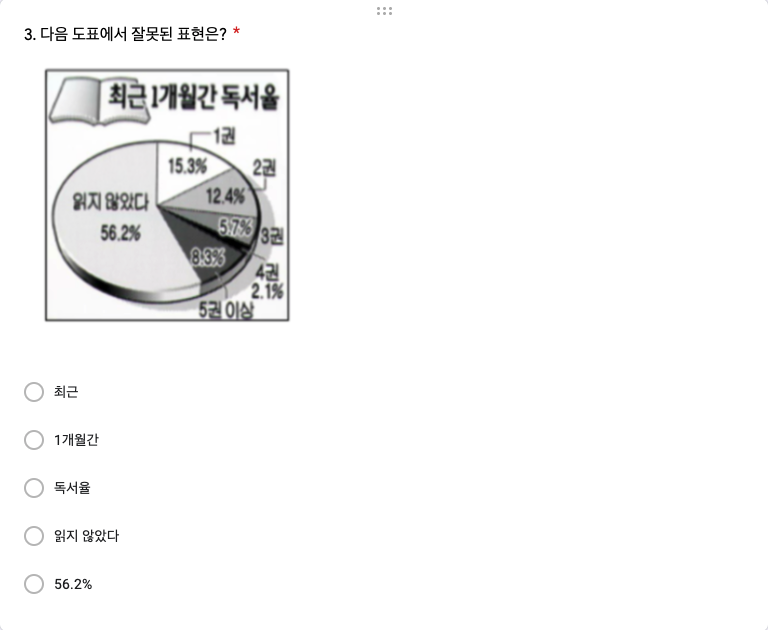
\includegraphics[width=0.75\linewidth]{./pics/Quiz210330_Q3} \end{flushleft}

\subsubsection{집계}\label{uxc9d1uxacc4-3}

\begin{longtable}[]{@{}
  >{\raggedright\arraybackslash}p{(\columnwidth - 12\tabcolsep) * \real{0.1667}}
  >{\centering\arraybackslash}p{(\columnwidth - 12\tabcolsep) * \real{0.0972}}
  >{\centering\arraybackslash}p{(\columnwidth - 12\tabcolsep) * \real{0.1389}}
  >{\centering\arraybackslash}p{(\columnwidth - 12\tabcolsep) * \real{0.1250}}
  >{\centering\arraybackslash}p{(\columnwidth - 12\tabcolsep) * \real{0.1944}}
  >{\raggedleft\arraybackslash}p{(\columnwidth - 12\tabcolsep) * \real{0.1111}}
  >{\centering\arraybackslash}p{(\columnwidth - 12\tabcolsep) * \real{0.1111}}@{}}
\toprule\noalign{}
\begin{minipage}[b]{\linewidth}\raggedright
~
\end{minipage} & \begin{minipage}[b]{\linewidth}\centering
최근
\end{minipage} & \begin{minipage}[b]{\linewidth}\centering
1개월간
\end{minipage} & \begin{minipage}[b]{\linewidth}\centering
독서율
\end{minipage} & \begin{minipage}[b]{\linewidth}\centering
읽지 않았다
\end{minipage} & \begin{minipage}[b]{\linewidth}\raggedleft
56.2\%
\end{minipage} & \begin{minipage}[b]{\linewidth}\centering
계
\end{minipage} \\
\midrule\noalign{}
\endhead
\bottomrule\noalign{}
\endlastfoot
\textbf{Red} & 15 & 13 & 137 & 11 & 11 & 187 \\
\textbf{Black} & 29 & 5 & 130 & 9 & 12 & 185 \\
\textbf{계} & 44 & 18 & 267 & 20 & 23 & 372 \\
\end{longtable}

\begin{longtable}[]{@{}
  >{\raggedleft\arraybackslash}p{(\columnwidth - 4\tabcolsep) * \real{0.2361}}
  >{\raggedleft\arraybackslash}p{(\columnwidth - 4\tabcolsep) * \real{0.0694}}
  >{\raggedleft\arraybackslash}p{(\columnwidth - 4\tabcolsep) * \real{0.1389}}@{}}
\caption{Pearson's Chi-squared test: \texttt{.}}\tabularnewline
\toprule\noalign{}
\begin{minipage}[b]{\linewidth}\raggedleft
Test statistic
\end{minipage} & \begin{minipage}[b]{\linewidth}\raggedleft
df
\end{minipage} & \begin{minipage}[b]{\linewidth}\raggedleft
P value
\end{minipage} \\
\midrule\noalign{}
\endfirsthead
\toprule\noalign{}
\begin{minipage}[b]{\linewidth}\raggedleft
Test statistic
\end{minipage} & \begin{minipage}[b]{\linewidth}\raggedleft
df
\end{minipage} & \begin{minipage}[b]{\linewidth}\raggedleft
P value
\end{minipage} \\
\midrule\noalign{}
\endhead
\bottomrule\noalign{}
\endlastfoot
8.427 & 4 & 0.07714 \\
\end{longtable}

Q4의 집계 결과가 Red, Black 간에 통계적으로 유의한 차이가 있는지
알아보기 위하여 카이제곱 테스트를 수행하였습니다.

그 결과 카이제곱 통계량은 8.43, 자유도는 4, p-value 는 0.0771이므로 Red,
Black 간에 통계적으로 유의한 차이를 보이지 않습니다.

실제로 닮은 게 느껴집니까?

\subsubsection{\%}\label{section-3}

\begin{longtable}[]{@{}
  >{\centering\arraybackslash}p{(\columnwidth - 10\tabcolsep) * \real{0.0972}}
  >{\centering\arraybackslash}p{(\columnwidth - 10\tabcolsep) * \real{0.1389}}
  >{\centering\arraybackslash}p{(\columnwidth - 10\tabcolsep) * \real{0.1250}}
  >{\centering\arraybackslash}p{(\columnwidth - 10\tabcolsep) * \real{0.1944}}
  >{\raggedleft\arraybackslash}p{(\columnwidth - 10\tabcolsep) * \real{0.1111}}
  >{\centering\arraybackslash}p{(\columnwidth - 10\tabcolsep) * \real{0.1111}}@{}}
\toprule\noalign{}
\begin{minipage}[b]{\linewidth}\centering
최근
\end{minipage} & \begin{minipage}[b]{\linewidth}\centering
1개월간
\end{minipage} & \begin{minipage}[b]{\linewidth}\centering
독서율
\end{minipage} & \begin{minipage}[b]{\linewidth}\centering
읽지 않았다
\end{minipage} & \begin{minipage}[b]{\linewidth}\raggedleft
56.2\%
\end{minipage} & \begin{minipage}[b]{\linewidth}\centering
계
\end{minipage} \\
\midrule\noalign{}
\endhead
\bottomrule\noalign{}
\endlastfoot
11.8 & 4.8 & 71.8 & 5.4 & 6.2 & 100.0 \\
\end{longtable}

정답률은 Red, Black 을 합하여 계산하는데, 71.8(\%) 입니다.

\subsection{Q5. 20대의
연간독서율}\label{q5.-20uxb300uxc758-uxc5f0uxac04uxb3c5uxc11cuxc728}

\begin{flushleft}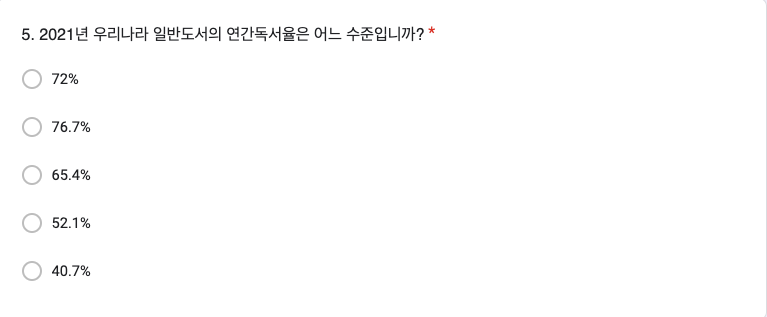
\includegraphics[width=0.75\linewidth]{./pics/Quiz230405_Q5} \end{flushleft}

\subsubsection{집계}\label{uxc9d1uxacc4-4}

\begin{longtable}[]{@{}
  >{\raggedright\arraybackslash}p{(\columnwidth - 12\tabcolsep) * \real{0.1667}}
  >{\raggedleft\arraybackslash}p{(\columnwidth - 12\tabcolsep) * \real{0.1111}}
  >{\raggedleft\arraybackslash}p{(\columnwidth - 12\tabcolsep) * \real{0.1111}}
  >{\raggedleft\arraybackslash}p{(\columnwidth - 12\tabcolsep) * \real{0.1111}}
  >{\raggedleft\arraybackslash}p{(\columnwidth - 12\tabcolsep) * \real{0.1111}}
  >{\raggedleft\arraybackslash}p{(\columnwidth - 12\tabcolsep) * \real{0.1111}}
  >{\centering\arraybackslash}p{(\columnwidth - 12\tabcolsep) * \real{0.1111}}@{}}
\toprule\noalign{}
\begin{minipage}[b]{\linewidth}\raggedright
~
\end{minipage} & \begin{minipage}[b]{\linewidth}\raggedleft
72.0\%
\end{minipage} & \begin{minipage}[b]{\linewidth}\raggedleft
76.7\%
\end{minipage} & \begin{minipage}[b]{\linewidth}\raggedleft
65.4\%
\end{minipage} & \begin{minipage}[b]{\linewidth}\raggedleft
52.1\%
\end{minipage} & \begin{minipage}[b]{\linewidth}\raggedleft
40.7\%
\end{minipage} & \begin{minipage}[b]{\linewidth}\centering
계
\end{minipage} \\
\midrule\noalign{}
\endhead
\bottomrule\noalign{}
\endlastfoot
\textbf{Red} & 4 & 8 & 17 & 26 & 132 & 187 \\
\textbf{Black} & 3 & 10 & 16 & 31 & 125 & 185 \\
\textbf{계} & 7 & 18 & 33 & 57 & 257 & 372 \\
\end{longtable}

\begin{longtable}[]{@{}
  >{\raggedleft\arraybackslash}p{(\columnwidth - 4\tabcolsep) * \real{0.2361}}
  >{\raggedleft\arraybackslash}p{(\columnwidth - 4\tabcolsep) * \real{0.0694}}
  >{\raggedleft\arraybackslash}p{(\columnwidth - 4\tabcolsep) * \real{0.1389}}@{}}
\caption{Pearson's Chi-squared test: \texttt{.}}\tabularnewline
\toprule\noalign{}
\begin{minipage}[b]{\linewidth}\raggedleft
Test statistic
\end{minipage} & \begin{minipage}[b]{\linewidth}\raggedleft
df
\end{minipage} & \begin{minipage}[b]{\linewidth}\raggedleft
P value
\end{minipage} \\
\midrule\noalign{}
\endfirsthead
\toprule\noalign{}
\begin{minipage}[b]{\linewidth}\raggedleft
Test statistic
\end{minipage} & \begin{minipage}[b]{\linewidth}\raggedleft
df
\end{minipage} & \begin{minipage}[b]{\linewidth}\raggedleft
P value
\end{minipage} \\
\midrule\noalign{}
\endhead
\bottomrule\noalign{}
\endlastfoot
1.014 & 4 & 0.9077 \\
\end{longtable}

Q5의 집계 결과가 Red, Black 간에 통계적으로 유의한 차이가 있는지
알아보기 위하여 카이제곱 테스트를 수행하였습니다.

그 결과 카이제곱 통계량은 1.01, 자유도는 4, p-value 는 0.9077이므로 Red,
Black 간에 통계적으로 유의한 차이를 보이지 않습니다.

실제로 닮은 게 느껴집니까?

\subsubsection{\%}\label{section-4}

\begin{longtable}[]{@{}
  >{\raggedleft\arraybackslash}p{(\columnwidth - 10\tabcolsep) * \real{0.1111}}
  >{\raggedleft\arraybackslash}p{(\columnwidth - 10\tabcolsep) * \real{0.1111}}
  >{\raggedleft\arraybackslash}p{(\columnwidth - 10\tabcolsep) * \real{0.1111}}
  >{\raggedleft\arraybackslash}p{(\columnwidth - 10\tabcolsep) * \real{0.1111}}
  >{\raggedleft\arraybackslash}p{(\columnwidth - 10\tabcolsep) * \real{0.1111}}
  >{\centering\arraybackslash}p{(\columnwidth - 10\tabcolsep) * \real{0.1111}}@{}}
\toprule\noalign{}
\begin{minipage}[b]{\linewidth}\raggedleft
72.0\%
\end{minipage} & \begin{minipage}[b]{\linewidth}\raggedleft
76.7\%
\end{minipage} & \begin{minipage}[b]{\linewidth}\raggedleft
65.4\%
\end{minipage} & \begin{minipage}[b]{\linewidth}\raggedleft
52.1\%
\end{minipage} & \begin{minipage}[b]{\linewidth}\raggedleft
40.7\%
\end{minipage} & \begin{minipage}[b]{\linewidth}\centering
계
\end{minipage} \\
\midrule\noalign{}
\endhead
\bottomrule\noalign{}
\endlastfoot
1.9 & 4.8 & 8.9 & 15.3 & 69.1 & 100.0 \\
\end{longtable}

정답률은 Red, Black 을 합하여 계산하는데, 69.1(\%) 입니다.

\subsection{Q6. 50대의
연간독서율}\label{q6.-50uxb300uxc758-uxc5f0uxac04uxb3c5uxc11cuxc728}

\begin{flushleft}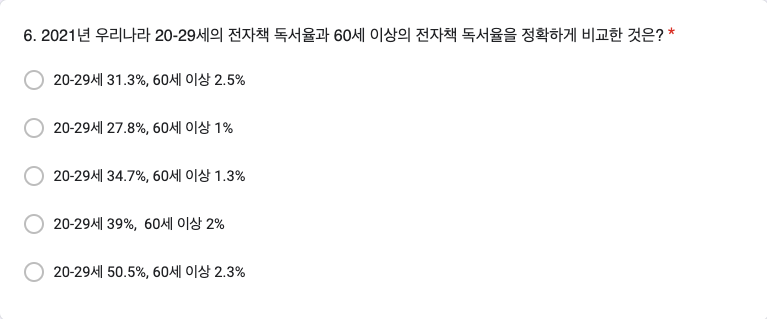
\includegraphics[width=0.75\linewidth]{./pics/Quiz230405_Q6} \end{flushleft}

\subsubsection{집계}\label{uxc9d1uxacc4-5}

\begin{longtable}[]{@{}
  >{\raggedright\arraybackslash}p{(\columnwidth - 12\tabcolsep) * \real{0.0764}}
  >{\centering\arraybackslash}p{(\columnwidth - 12\tabcolsep) * \real{0.1783}}
  >{\centering\arraybackslash}p{(\columnwidth - 12\tabcolsep) * \real{0.1783}}
  >{\centering\arraybackslash}p{(\columnwidth - 12\tabcolsep) * \real{0.1783}}
  >{\centering\arraybackslash}p{(\columnwidth - 12\tabcolsep) * \real{0.1720}}
  >{\centering\arraybackslash}p{(\columnwidth - 12\tabcolsep) * \real{0.1783}}
  >{\centering\arraybackslash}p{(\columnwidth - 12\tabcolsep) * \real{0.0382}}@{}}
\toprule\noalign{}
\begin{minipage}[b]{\linewidth}\raggedright
~
\end{minipage} & \begin{minipage}[b]{\linewidth}\centering
20-29세 31.3\%, 60세 이상 2.5\%
\end{minipage} & \begin{minipage}[b]{\linewidth}\centering
20-29세 27.8\%, 60세 이상 1\%
\end{minipage} & \begin{minipage}[b]{\linewidth}\centering
20-29세 34.7\%, 60세 이상 1.3\%
\end{minipage} & \begin{minipage}[b]{\linewidth}\centering
20-29세 39\%, 60세 이상 2\%
\end{minipage} & \begin{minipage}[b]{\linewidth}\centering
20-29세 50.5\%, 60세 이상 2.3\%
\end{minipage} & \begin{minipage}[b]{\linewidth}\centering
계
\end{minipage} \\
\midrule\noalign{}
\endhead
\bottomrule\noalign{}
\endlastfoot
\textbf{Red} & 19 & 24 & 28 & 15 & 101 & 187 \\
\textbf{Black} & 20 & 26 & 32 & 12 & 95 & 185 \\
\textbf{계} & 39 & 50 & 60 & 27 & 196 & 372 \\
\end{longtable}

\begin{longtable}[]{@{}
  >{\raggedleft\arraybackslash}p{(\columnwidth - 4\tabcolsep) * \real{0.2361}}
  >{\raggedleft\arraybackslash}p{(\columnwidth - 4\tabcolsep) * \real{0.0694}}
  >{\raggedleft\arraybackslash}p{(\columnwidth - 4\tabcolsep) * \real{0.1389}}@{}}
\caption{Pearson's Chi-squared test: \texttt{.}}\tabularnewline
\toprule\noalign{}
\begin{minipage}[b]{\linewidth}\raggedleft
Test statistic
\end{minipage} & \begin{minipage}[b]{\linewidth}\raggedleft
df
\end{minipage} & \begin{minipage}[b]{\linewidth}\raggedleft
P value
\end{minipage} \\
\midrule\noalign{}
\endfirsthead
\toprule\noalign{}
\begin{minipage}[b]{\linewidth}\raggedleft
Test statistic
\end{minipage} & \begin{minipage}[b]{\linewidth}\raggedleft
df
\end{minipage} & \begin{minipage}[b]{\linewidth}\raggedleft
P value
\end{minipage} \\
\midrule\noalign{}
\endhead
\bottomrule\noalign{}
\endlastfoot
0.8786 & 4 & 0.9276 \\
\end{longtable}

Q6의 집계 결과가 Red, Black 간에 통계적으로 유의한 차이가 있는지
알아보기 위하여 카이제곱 테스트를 수행하였습니다.

그 결과 카이제곱 통계량은 0.88, 자유도는 4, p-value 는 0.9276이므로 Red,
Black 간에 통계적으로 유의한 차이를 보이지 않습니다.

실제로 닮은 게 느껴집니까?

\subsubsection{\%}\label{section-5}

\begin{longtable}[]{@{}
  >{\centering\arraybackslash}p{(\columnwidth - 10\tabcolsep) * \real{0.1905}}
  >{\centering\arraybackslash}p{(\columnwidth - 10\tabcolsep) * \real{0.1905}}
  >{\centering\arraybackslash}p{(\columnwidth - 10\tabcolsep) * \real{0.1905}}
  >{\centering\arraybackslash}p{(\columnwidth - 10\tabcolsep) * \real{0.1837}}
  >{\centering\arraybackslash}p{(\columnwidth - 10\tabcolsep) * \real{0.1905}}
  >{\centering\arraybackslash}p{(\columnwidth - 10\tabcolsep) * \real{0.0544}}@{}}
\toprule\noalign{}
\begin{minipage}[b]{\linewidth}\centering
20-29세 31.3\%, 60세 이상 2.5\%
\end{minipage} & \begin{minipage}[b]{\linewidth}\centering
20-29세 27.8\%, 60세 이상 1\%
\end{minipage} & \begin{minipage}[b]{\linewidth}\centering
20-29세 34.7\%, 60세 이상 1.3\%
\end{minipage} & \begin{minipage}[b]{\linewidth}\centering
20-29세 39\%, 60세 이상 2\%
\end{minipage} & \begin{minipage}[b]{\linewidth}\centering
20-29세 50.5\%, 60세 이상 2.3\%
\end{minipage} & \begin{minipage}[b]{\linewidth}\centering
계
\end{minipage} \\
\midrule\noalign{}
\endhead
\bottomrule\noalign{}
\endlastfoot
10.5 & 13.4 & 16.1 & 7.3 & 52.7 & 100.0 \\
\end{longtable}

정답률은 Red, Black 을 합하여 계산하는데, 52.7(\%) 입니다.

\subsection{Q7. The more, the better? : 내가 남보다, 혹은 남이
나보다}\label{q7.-the-more-the-better-uxb0b4uxac00-uxb0a8uxbcf4uxb2e4-uxd639uxc740-uxb0a8uxc774-uxb098uxbcf4uxb2e4}

Q7의 응답결과는 매우 중요한 시사점을 보여줍니다.

다다익선, 많으면 많을수록 좋다, 영어로는 The more, the better 가 아니라
절대 금액은 적더라도 상대적 비교에서 많은 것을 더 선호한다는 것입니다.

Red 와 Black 의 차이는 순서를 바꿔서 소위 1번효과가 나타나는지를
살펴보고자 하였으나 P-value 가 시사하듯이 그러한 차이는 관찰되지
않습니다.

소득의 절대값이 아니라 상대 비교가 중요하다는 Solnick and
Hemenway(1998)의 연구결과와 일치합니다.

랜덤화하였지만 응답에는 차이가 없음을 보여주고 있습니다.

\begin{flushleft}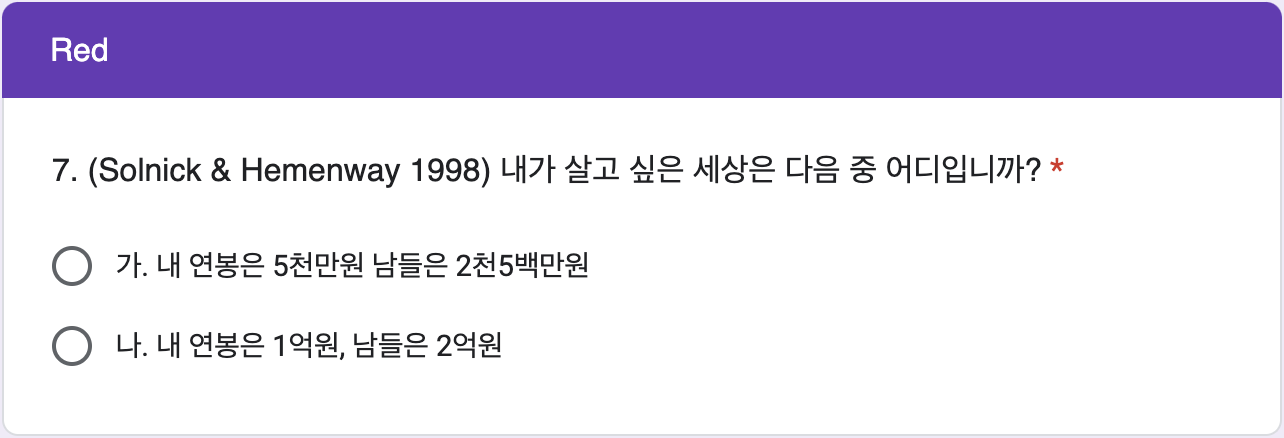
\includegraphics[width=0.67\linewidth]{./pics/Quiz240405_Q7_Red} \end{flushleft}

\begin{flushleft}
\includegraphics[width=0.67\linewidth]{./pics/Quiz240405_Q7_Black} \end{flushleft}

\subsubsection{집계}\label{uxc9d1uxacc4-6}

\begin{longtable}[]{@{}
  >{\raggedright\arraybackslash}p{(\columnwidth - 6\tabcolsep) * \real{0.4444}}
  >{\centering\arraybackslash}p{(\columnwidth - 6\tabcolsep) * \real{0.1944}}
  >{\centering\arraybackslash}p{(\columnwidth - 6\tabcolsep) * \real{0.1944}}
  >{\centering\arraybackslash}p{(\columnwidth - 6\tabcolsep) * \real{0.0833}}@{}}
\toprule\noalign{}
\begin{minipage}[b]{\linewidth}\raggedright
~
\end{minipage} & \begin{minipage}[b]{\linewidth}\centering
내가 남보다
\end{minipage} & \begin{minipage}[b]{\linewidth}\centering
남이 나보다
\end{minipage} & \begin{minipage}[b]{\linewidth}\centering
계
\end{minipage} \\
\midrule\noalign{}
\endhead
\bottomrule\noalign{}
\endlastfoot
\textbf{Red(`내가 남보다' 먼저)} & 138 & 49 & 187 \\
\textbf{Black(`남이 나보다' 먼저)} & 139 & 46 & 185 \\
\textbf{계} & 277 & 95 & 372 \\
\end{longtable}

\begin{longtable}[]{@{}
  >{\raggedleft\arraybackslash}p{(\columnwidth - 4\tabcolsep) * \real{0.2361}}
  >{\raggedleft\arraybackslash}p{(\columnwidth - 4\tabcolsep) * \real{0.0694}}
  >{\raggedleft\arraybackslash}p{(\columnwidth - 4\tabcolsep) * \real{0.1389}}@{}}
\caption{Pearson's Chi-squared test with Yates' continuity correction:
\texttt{.}}\tabularnewline
\toprule\noalign{}
\begin{minipage}[b]{\linewidth}\raggedleft
Test statistic
\end{minipage} & \begin{minipage}[b]{\linewidth}\raggedleft
df
\end{minipage} & \begin{minipage}[b]{\linewidth}\raggedleft
P value
\end{minipage} \\
\midrule\noalign{}
\endfirsthead
\toprule\noalign{}
\begin{minipage}[b]{\linewidth}\raggedleft
Test statistic
\end{minipage} & \begin{minipage}[b]{\linewidth}\raggedleft
df
\end{minipage} & \begin{minipage}[b]{\linewidth}\raggedleft
P value
\end{minipage} \\
\midrule\noalign{}
\endhead
\bottomrule\noalign{}
\endlastfoot
0.03135 & 1 & 0.8595 \\
\end{longtable}

Q7의 Red 는 앞 선택지에 내 연봉은 5천만원, 남들은 2천5백만원을 받는
세상을 제시하고 뒷 선택지에 내 연봉은 1억원, 남들은 2억원을 받는 세상을
제시하였습니다.

Black 은 각 선택지의 순서만 바꿔서 소위 1번효과를 측정하려 하였습니다.

집계결과는 절대금액에서 많이 받는 세상보다 상대적으로 더 많이 받는
세상을 원한다는 점을 명확히 보여 줍니다.

여기서 수행하고 있는 카이제곱 테스트는 선택지의 순서만 바꿨을 때
통계적으로 유의한 차이를 보여주는지 파악하는 것으로서 카이제곱 통계량은
0.031, 자유도는 1, p-value 는 0.8595로 깜짝 놀랄만큼 선택지의 순서는
관계 없다는 것을 보여 줍니다.

여러분이 보기에도 그렇게 닮았다고 느껴집니까?

이번에도 귀류법의 논리를 적용해 봅니다.

여기서 선택지의 순서를 바꾸는 것이 응답에 영향을 끼치지 않는다고 가정해
봅시다.

그렇다면 Red, Black 의 응답은 Q1\textasciitilde Q4 에서와 같이 랜덤화
효과에 의하여 통계적으로 유의한 차이를 보이지 않을 것입니다.

그리고 실제로 관찰된 카이제곱 통계값의 p-value 도 0.05와는 비교도 안
되는 수준으로 크기 때문에 통계적으로 유의한 차이를 보여주지 못합니다.

따라서 선지의 순서를 바꾸는 것은 응답에 영향을 끼치지 못한다는 가설을
받아들이게 됩니다.

\subsubsection{\% 비교.}\label{uxbe44uxad50.}

\begin{longtable}[]{@{}
  >{\raggedright\arraybackslash}p{(\columnwidth - 6\tabcolsep) * \real{0.4444}}
  >{\centering\arraybackslash}p{(\columnwidth - 6\tabcolsep) * \real{0.1944}}
  >{\centering\arraybackslash}p{(\columnwidth - 6\tabcolsep) * \real{0.1944}}
  >{\centering\arraybackslash}p{(\columnwidth - 6\tabcolsep) * \real{0.1111}}@{}}
\toprule\noalign{}
\begin{minipage}[b]{\linewidth}\raggedright
~
\end{minipage} & \begin{minipage}[b]{\linewidth}\centering
내가 남보다
\end{minipage} & \begin{minipage}[b]{\linewidth}\centering
남이 나보다
\end{minipage} & \begin{minipage}[b]{\linewidth}\centering
계
\end{minipage} \\
\midrule\noalign{}
\endhead
\bottomrule\noalign{}
\endlastfoot
\textbf{Red(`내가 남보다' 먼저)} & 73.8 & 26.2 & 100.0 \\
\textbf{Black(`남이 나보다' 먼저)} & 75.1 & 24.9 & 100.0 \\
\end{longtable}

이를 백분율로 살펴보면 ``내가 남보다''를 앞 선택지로 한 Red 에서 ``내가
남보다''를 선택한 백분율, 73.8(\%)(이)나 ``남이 나보다''를 앞에 앞
선택지로 한 Black 에서 ``내가 남보다''를 선택한 백분율, 75.1(\%)(이)나
거의 차이가 없어서 선택지의 순서를 바꿔 봐야 응답에 통계적으로 유의한
영향을 주지 못한다는 것을 명확히 알 수 있습니다.

따라서 통계적으로 유의한 차이를 관찰하지 못했으므로 Red, Black 은 합쳐서
분석하는 것이 타당합니다.

그 결과는 다음과 같습니다.

\subsubsection{합산(\%)}\label{uxd569uxc0b0}

\begin{longtable}[]{@{}
  >{\centering\arraybackslash}p{(\columnwidth - 4\tabcolsep) * \real{0.1944}}
  >{\centering\arraybackslash}p{(\columnwidth - 4\tabcolsep) * \real{0.1944}}
  >{\centering\arraybackslash}p{(\columnwidth - 4\tabcolsep) * \real{0.1111}}@{}}
\toprule\noalign{}
\begin{minipage}[b]{\linewidth}\centering
내가 남보다
\end{minipage} & \begin{minipage}[b]{\linewidth}\centering
남이 나보다
\end{minipage} & \begin{minipage}[b]{\linewidth}\centering
계
\end{minipage} \\
\midrule\noalign{}
\endhead
\bottomrule\noalign{}
\endlastfoot
74.5 & 25.5 & 100.0 \\
\end{longtable}

``내가 남보다'' 많이 받는 세상을 원한다고 응답한 백분률은 선택지의
순서와는 무관하게 74.5(\%)(으)로 매우 높습니다.

\subsubsection{Mosaic Plot}\label{mosaic-plot}


\includegraphics{quiz250407_Report_v4_files/figure-latex/mosaic plot-1.pdf}

Mosaic Plot 은 이 집계결과를 시각적으로 잘 보여줍니다.

선택지의 순서에 거의 무관할 정도로 응답이 비슷하기 때문에 Red, Black 이
닮았고, ``내가 남보다'' 많이 받아야 한다고 응답한 백분율도 닮은 것을 잘
알 수 있습니다.

\subsection{마감 시간으로부터 제출 시간의
분포}\label{uxb9c8uxac10-uxc2dcuxac04uxc73cuxb85cuxbd80uxd130-uxc81cuxcd9c-uxc2dcuxac04uxc758-uxbd84uxd3ec}

\subsubsection{분포표}\label{uxbd84uxd3ecuxd45c}

\begin{longtable}[]{@{}
  >{\raggedright\arraybackslash}p{(\columnwidth - 30\tabcolsep) * \real{0.0863}}
  >{\raggedleft\arraybackslash}p{(\columnwidth - 30\tabcolsep) * \real{0.0576}}
  >{\raggedleft\arraybackslash}p{(\columnwidth - 30\tabcolsep) * \real{0.0576}}
  >{\raggedleft\arraybackslash}p{(\columnwidth - 30\tabcolsep) * \real{0.0576}}
  >{\raggedleft\arraybackslash}p{(\columnwidth - 30\tabcolsep) * \real{0.0576}}
  >{\raggedleft\arraybackslash}p{(\columnwidth - 30\tabcolsep) * \real{0.0576}}
  >{\raggedleft\arraybackslash}p{(\columnwidth - 30\tabcolsep) * \real{0.0576}}
  >{\raggedleft\arraybackslash}p{(\columnwidth - 30\tabcolsep) * \real{0.0576}}
  >{\raggedleft\arraybackslash}p{(\columnwidth - 30\tabcolsep) * \real{0.0576}}
  >{\raggedleft\arraybackslash}p{(\columnwidth - 30\tabcolsep) * \real{0.0576}}
  >{\raggedleft\arraybackslash}p{(\columnwidth - 30\tabcolsep) * \real{0.0647}}
  >{\raggedleft\arraybackslash}p{(\columnwidth - 30\tabcolsep) * \real{0.0719}}
  >{\raggedleft\arraybackslash}p{(\columnwidth - 30\tabcolsep) * \real{0.0719}}
  >{\raggedleft\arraybackslash}p{(\columnwidth - 30\tabcolsep) * \real{0.0719}}
  >{\raggedleft\arraybackslash}p{(\columnwidth - 30\tabcolsep) * \real{0.0719}}
  >{\centering\arraybackslash}p{(\columnwidth - 30\tabcolsep) * \real{0.0432}}@{}}
\caption{일 단위}\tabularnewline
\toprule\noalign{}
\begin{minipage}[b]{\linewidth}\raggedright
~
\end{minipage} & \begin{minipage}[b]{\linewidth}\raggedleft
{[}0,1{]}
\end{minipage} & \begin{minipage}[b]{\linewidth}\raggedleft
(1,2{]}
\end{minipage} & \begin{minipage}[b]{\linewidth}\raggedleft
(2,3{]}
\end{minipage} & \begin{minipage}[b]{\linewidth}\raggedleft
(3,4{]}
\end{minipage} & \begin{minipage}[b]{\linewidth}\raggedleft
(4,5{]}
\end{minipage} & \begin{minipage}[b]{\linewidth}\raggedleft
(5,6{]}
\end{minipage} & \begin{minipage}[b]{\linewidth}\raggedleft
(6,7{]}
\end{minipage} & \begin{minipage}[b]{\linewidth}\raggedleft
(7,8{]}
\end{minipage} & \begin{minipage}[b]{\linewidth}\raggedleft
(8,9{]}
\end{minipage} & \begin{minipage}[b]{\linewidth}\raggedleft
(9,10{]}
\end{minipage} & \begin{minipage}[b]{\linewidth}\raggedleft
(10,11{]}
\end{minipage} & \begin{minipage}[b]{\linewidth}\raggedleft
(11,12{]}
\end{minipage} & \begin{minipage}[b]{\linewidth}\raggedleft
(12,13{]}
\end{minipage} & \begin{minipage}[b]{\linewidth}\raggedleft
(13,14{]}
\end{minipage} & \begin{minipage}[b]{\linewidth}\centering
계
\end{minipage} \\
\midrule\noalign{}
\endfirsthead
\toprule\noalign{}
\begin{minipage}[b]{\linewidth}\raggedright
~
\end{minipage} & \begin{minipage}[b]{\linewidth}\raggedleft
{[}0,1{]}
\end{minipage} & \begin{minipage}[b]{\linewidth}\raggedleft
(1,2{]}
\end{minipage} & \begin{minipage}[b]{\linewidth}\raggedleft
(2,3{]}
\end{minipage} & \begin{minipage}[b]{\linewidth}\raggedleft
(3,4{]}
\end{minipage} & \begin{minipage}[b]{\linewidth}\raggedleft
(4,5{]}
\end{minipage} & \begin{minipage}[b]{\linewidth}\raggedleft
(5,6{]}
\end{minipage} & \begin{minipage}[b]{\linewidth}\raggedleft
(6,7{]}
\end{minipage} & \begin{minipage}[b]{\linewidth}\raggedleft
(7,8{]}
\end{minipage} & \begin{minipage}[b]{\linewidth}\raggedleft
(8,9{]}
\end{minipage} & \begin{minipage}[b]{\linewidth}\raggedleft
(9,10{]}
\end{minipage} & \begin{minipage}[b]{\linewidth}\raggedleft
(10,11{]}
\end{minipage} & \begin{minipage}[b]{\linewidth}\raggedleft
(11,12{]}
\end{minipage} & \begin{minipage}[b]{\linewidth}\raggedleft
(12,13{]}
\end{minipage} & \begin{minipage}[b]{\linewidth}\raggedleft
(13,14{]}
\end{minipage} & \begin{minipage}[b]{\linewidth}\centering
계
\end{minipage} \\
\midrule\noalign{}
\endhead
\bottomrule\noalign{}
\endlastfoot
\textbf{Red} & 0 & 1 & 10 & 6 & 4 & 6 & 9 & 35 & 20 & 16 & 10 & 26 & 18
& 26 & 187 \\
\textbf{Black} & 0 & 1 & 8 & 3 & 3 & 7 & 11 & 47 & 16 & 14 & 15 & 14 &
21 & 25 & 185 \\
\textbf{계} & 0 & 2 & 18 & 9 & 7 & 13 & 20 & 82 & 36 & 30 & 25 & 40 & 39
& 51 & 372 \\
\end{longtable}

분포표로부터 두 가지 문제를 살펴보겠습니다.

첫째, 날마다 고르게 제출하는가?

둘째, Red, Black 간에 통계적으로 유의한 차이가 있는가?

각 문제를 살펴보기 위해서는 분포표의 일부분을 대상으로 카이제곱 테스트를
수행합니다.

\subsubsection{날마다 고르게
제출하는가?}\label{uxb0a0uxb9c8uxb2e4-uxace0uxb974uxac8c-uxc81cuxcd9cuxd558uxb294uxac00}

\begin{longtable}[]{@{}
  >{\raggedleft\arraybackslash}p{(\columnwidth - 24\tabcolsep) * \real{0.0708}}
  >{\raggedleft\arraybackslash}p{(\columnwidth - 24\tabcolsep) * \real{0.0708}}
  >{\raggedleft\arraybackslash}p{(\columnwidth - 24\tabcolsep) * \real{0.0708}}
  >{\raggedleft\arraybackslash}p{(\columnwidth - 24\tabcolsep) * \real{0.0708}}
  >{\raggedleft\arraybackslash}p{(\columnwidth - 24\tabcolsep) * \real{0.0708}}
  >{\raggedleft\arraybackslash}p{(\columnwidth - 24\tabcolsep) * \real{0.0708}}
  >{\raggedleft\arraybackslash}p{(\columnwidth - 24\tabcolsep) * \real{0.0708}}
  >{\raggedleft\arraybackslash}p{(\columnwidth - 24\tabcolsep) * \real{0.0708}}
  >{\raggedleft\arraybackslash}p{(\columnwidth - 24\tabcolsep) * \real{0.0796}}
  >{\raggedleft\arraybackslash}p{(\columnwidth - 24\tabcolsep) * \real{0.0885}}
  >{\raggedleft\arraybackslash}p{(\columnwidth - 24\tabcolsep) * \real{0.0885}}
  >{\raggedleft\arraybackslash}p{(\columnwidth - 24\tabcolsep) * \real{0.0885}}
  >{\raggedleft\arraybackslash}p{(\columnwidth - 24\tabcolsep) * \real{0.0885}}@{}}
\toprule\noalign{}
\begin{minipage}[b]{\linewidth}\raggedleft
(1,2{]}
\end{minipage} & \begin{minipage}[b]{\linewidth}\raggedleft
(2,3{]}
\end{minipage} & \begin{minipage}[b]{\linewidth}\raggedleft
(3,4{]}
\end{minipage} & \begin{minipage}[b]{\linewidth}\raggedleft
(4,5{]}
\end{minipage} & \begin{minipage}[b]{\linewidth}\raggedleft
(5,6{]}
\end{minipage} & \begin{minipage}[b]{\linewidth}\raggedleft
(6,7{]}
\end{minipage} & \begin{minipage}[b]{\linewidth}\raggedleft
(7,8{]}
\end{minipage} & \begin{minipage}[b]{\linewidth}\raggedleft
(8,9{]}
\end{minipage} & \begin{minipage}[b]{\linewidth}\raggedleft
(9,10{]}
\end{minipage} & \begin{minipage}[b]{\linewidth}\raggedleft
(10,11{]}
\end{minipage} & \begin{minipage}[b]{\linewidth}\raggedleft
(11,12{]}
\end{minipage} & \begin{minipage}[b]{\linewidth}\raggedleft
(12,13{]}
\end{minipage} & \begin{minipage}[b]{\linewidth}\raggedleft
(13,14{]}
\end{minipage} \\
\midrule\noalign{}
\endhead
\bottomrule\noalign{}
\endlastfoot
2 & 18 & 9 & 7 & 13 & 20 & 82 & 36 & 30 & 25 & 40 & 39 & 51 \\
\end{longtable}

\begin{longtable}[]{@{}
  >{\raggedleft\arraybackslash}p{(\columnwidth - 4\tabcolsep) * \real{0.2361}}
  >{\raggedleft\arraybackslash}p{(\columnwidth - 4\tabcolsep) * \real{0.0694}}
  >{\raggedleft\arraybackslash}p{(\columnwidth - 4\tabcolsep) * \real{0.2500}}@{}}
\caption{Chi-squared test for given probabilities:
\texttt{.}}\tabularnewline
\toprule\noalign{}
\begin{minipage}[b]{\linewidth}\raggedleft
Test statistic
\end{minipage} & \begin{minipage}[b]{\linewidth}\raggedleft
df
\end{minipage} & \begin{minipage}[b]{\linewidth}\raggedleft
P value
\end{minipage} \\
\midrule\noalign{}
\endfirsthead
\toprule\noalign{}
\begin{minipage}[b]{\linewidth}\raggedleft
Test statistic
\end{minipage} & \begin{minipage}[b]{\linewidth}\raggedleft
df
\end{minipage} & \begin{minipage}[b]{\linewidth}\raggedleft
P value
\end{minipage} \\
\midrule\noalign{}
\endhead
\bottomrule\noalign{}
\endlastfoot
197.4 & 12 & 1.114e-35 * * * \\
\end{longtable}

날마다 고르게 제출하는지 알아 보았습니다.

분포표의 ``계''행에서 '계'열을 제외하고 카이제곱테스트를 수행합니다.

분포표 만으로도 쉽게 파악할 수 있지만 카이제곱테스트가 명확히 해 줍니다.

카이제곱 통계량은 197.41, 자유도는 12.00, p-value 는 1.1e-35 이므로
날짜별로 고르게 제출하고 있는지 살펴보기에는 천문학적으로 낮은 P-value
가 관찰되었습니다.

막대그래프로 살펴 보겠습니다.

\subsubsection{막대그래프}\label{uxb9c9uxb300uxadf8uxb798uxd504}

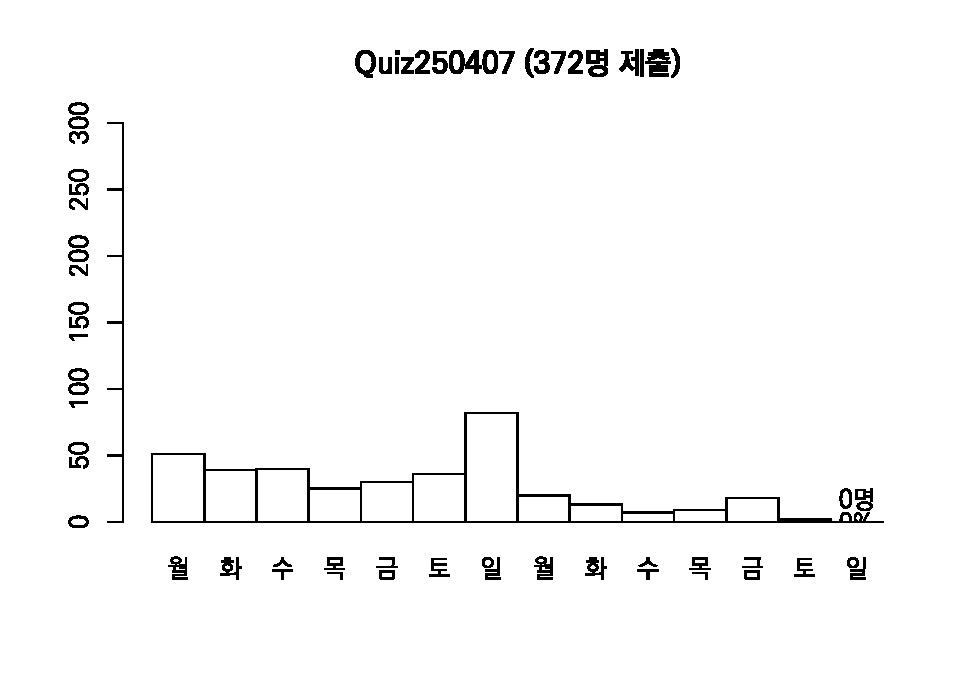
\includegraphics{quiz250407_Report_v4_files/figure-latex/unnamed-chunk-18-1.pdf}

\subsubsection{Red, Black 간에
닮았는가?}\label{red-black-uxac04uxc5d0-uxb2eeuxc558uxb294uxac00}

\begin{longtable}[]{@{}
  >{\raggedright\arraybackslash}p{(\columnwidth - 26\tabcolsep) * \real{0.0960}}
  >{\raggedleft\arraybackslash}p{(\columnwidth - 26\tabcolsep) * \real{0.0640}}
  >{\raggedleft\arraybackslash}p{(\columnwidth - 26\tabcolsep) * \real{0.0640}}
  >{\raggedleft\arraybackslash}p{(\columnwidth - 26\tabcolsep) * \real{0.0640}}
  >{\raggedleft\arraybackslash}p{(\columnwidth - 26\tabcolsep) * \real{0.0640}}
  >{\raggedleft\arraybackslash}p{(\columnwidth - 26\tabcolsep) * \real{0.0640}}
  >{\raggedleft\arraybackslash}p{(\columnwidth - 26\tabcolsep) * \real{0.0640}}
  >{\raggedleft\arraybackslash}p{(\columnwidth - 26\tabcolsep) * \real{0.0640}}
  >{\raggedleft\arraybackslash}p{(\columnwidth - 26\tabcolsep) * \real{0.0640}}
  >{\raggedleft\arraybackslash}p{(\columnwidth - 26\tabcolsep) * \real{0.0720}}
  >{\raggedleft\arraybackslash}p{(\columnwidth - 26\tabcolsep) * \real{0.0800}}
  >{\raggedleft\arraybackslash}p{(\columnwidth - 26\tabcolsep) * \real{0.0800}}
  >{\raggedleft\arraybackslash}p{(\columnwidth - 26\tabcolsep) * \real{0.0800}}
  >{\raggedleft\arraybackslash}p{(\columnwidth - 26\tabcolsep) * \real{0.0800}}@{}}
\toprule\noalign{}
\begin{minipage}[b]{\linewidth}\raggedright
~
\end{minipage} & \begin{minipage}[b]{\linewidth}\raggedleft
(1,2{]}
\end{minipage} & \begin{minipage}[b]{\linewidth}\raggedleft
(2,3{]}
\end{minipage} & \begin{minipage}[b]{\linewidth}\raggedleft
(3,4{]}
\end{minipage} & \begin{minipage}[b]{\linewidth}\raggedleft
(4,5{]}
\end{minipage} & \begin{minipage}[b]{\linewidth}\raggedleft
(5,6{]}
\end{minipage} & \begin{minipage}[b]{\linewidth}\raggedleft
(6,7{]}
\end{minipage} & \begin{minipage}[b]{\linewidth}\raggedleft
(7,8{]}
\end{minipage} & \begin{minipage}[b]{\linewidth}\raggedleft
(8,9{]}
\end{minipage} & \begin{minipage}[b]{\linewidth}\raggedleft
(9,10{]}
\end{minipage} & \begin{minipage}[b]{\linewidth}\raggedleft
(10,11{]}
\end{minipage} & \begin{minipage}[b]{\linewidth}\raggedleft
(11,12{]}
\end{minipage} & \begin{minipage}[b]{\linewidth}\raggedleft
(12,13{]}
\end{minipage} & \begin{minipage}[b]{\linewidth}\raggedleft
(13,14{]}
\end{minipage} \\
\midrule\noalign{}
\endhead
\bottomrule\noalign{}
\endlastfoot
\textbf{Red} & 1 & 10 & 6 & 4 & 6 & 9 & 35 & 20 & 16 & 10 & 26 & 18 &
26 \\
\textbf{Black} & 1 & 8 & 3 & 3 & 7 & 11 & 47 & 16 & 14 & 15 & 14 & 21 &
25 \\
\end{longtable}

\begin{longtable}[]{@{}
  >{\raggedleft\arraybackslash}p{(\columnwidth - 4\tabcolsep) * \real{0.2361}}
  >{\raggedleft\arraybackslash}p{(\columnwidth - 4\tabcolsep) * \real{0.0694}}
  >{\raggedleft\arraybackslash}p{(\columnwidth - 4\tabcolsep) * \real{0.1389}}@{}}
\caption{Pearson's Chi-squared test: \texttt{.}}\tabularnewline
\toprule\noalign{}
\begin{minipage}[b]{\linewidth}\raggedleft
Test statistic
\end{minipage} & \begin{minipage}[b]{\linewidth}\raggedleft
df
\end{minipage} & \begin{minipage}[b]{\linewidth}\raggedleft
P value
\end{minipage} \\
\midrule\noalign{}
\endfirsthead
\toprule\noalign{}
\begin{minipage}[b]{\linewidth}\raggedleft
Test statistic
\end{minipage} & \begin{minipage}[b]{\linewidth}\raggedleft
df
\end{minipage} & \begin{minipage}[b]{\linewidth}\raggedleft
P value
\end{minipage} \\
\midrule\noalign{}
\endhead
\bottomrule\noalign{}
\endlastfoot
8.816 & 12 & 0.7186 \\
\end{longtable}

제출시간의 분포가 Red, Black 간에 닮았는지 알아 보았습니다.

이번에는 분포표의 첫번째와 두번째 행, '계'열을 제외한 나머지 열에 대해서
카이제곱테스트를 수행합니다.

카이제곱 통계량은 8.82, 자유도는 12, p-value 는 0.72 이므로 제출 시간의
분포는 Red, Black 간에 통계적으로 유의한 차이가 관찰되고 있습니다.

이 사실을 Mosaic Plot 을 이용하여 시각적으로 살펴보겠습니다.

어디서 차이가 나고 있나요?

\subsubsection{Mosaic Plot}\label{mosaic-plot-1}


\includegraphics{quiz250407_Report_v4_files/figure-latex/unnamed-chunk-20-1.pdf}

\end{document}
